\documentclass{standalone}
\usepackage{tikz}
\usetikzlibrary{arrows.meta, bending, positioning, intersections, backgrounds}
\tikzset{x=0.6cm,y=0.6cm, >={Stealth[bend]}}

\begin{document}  
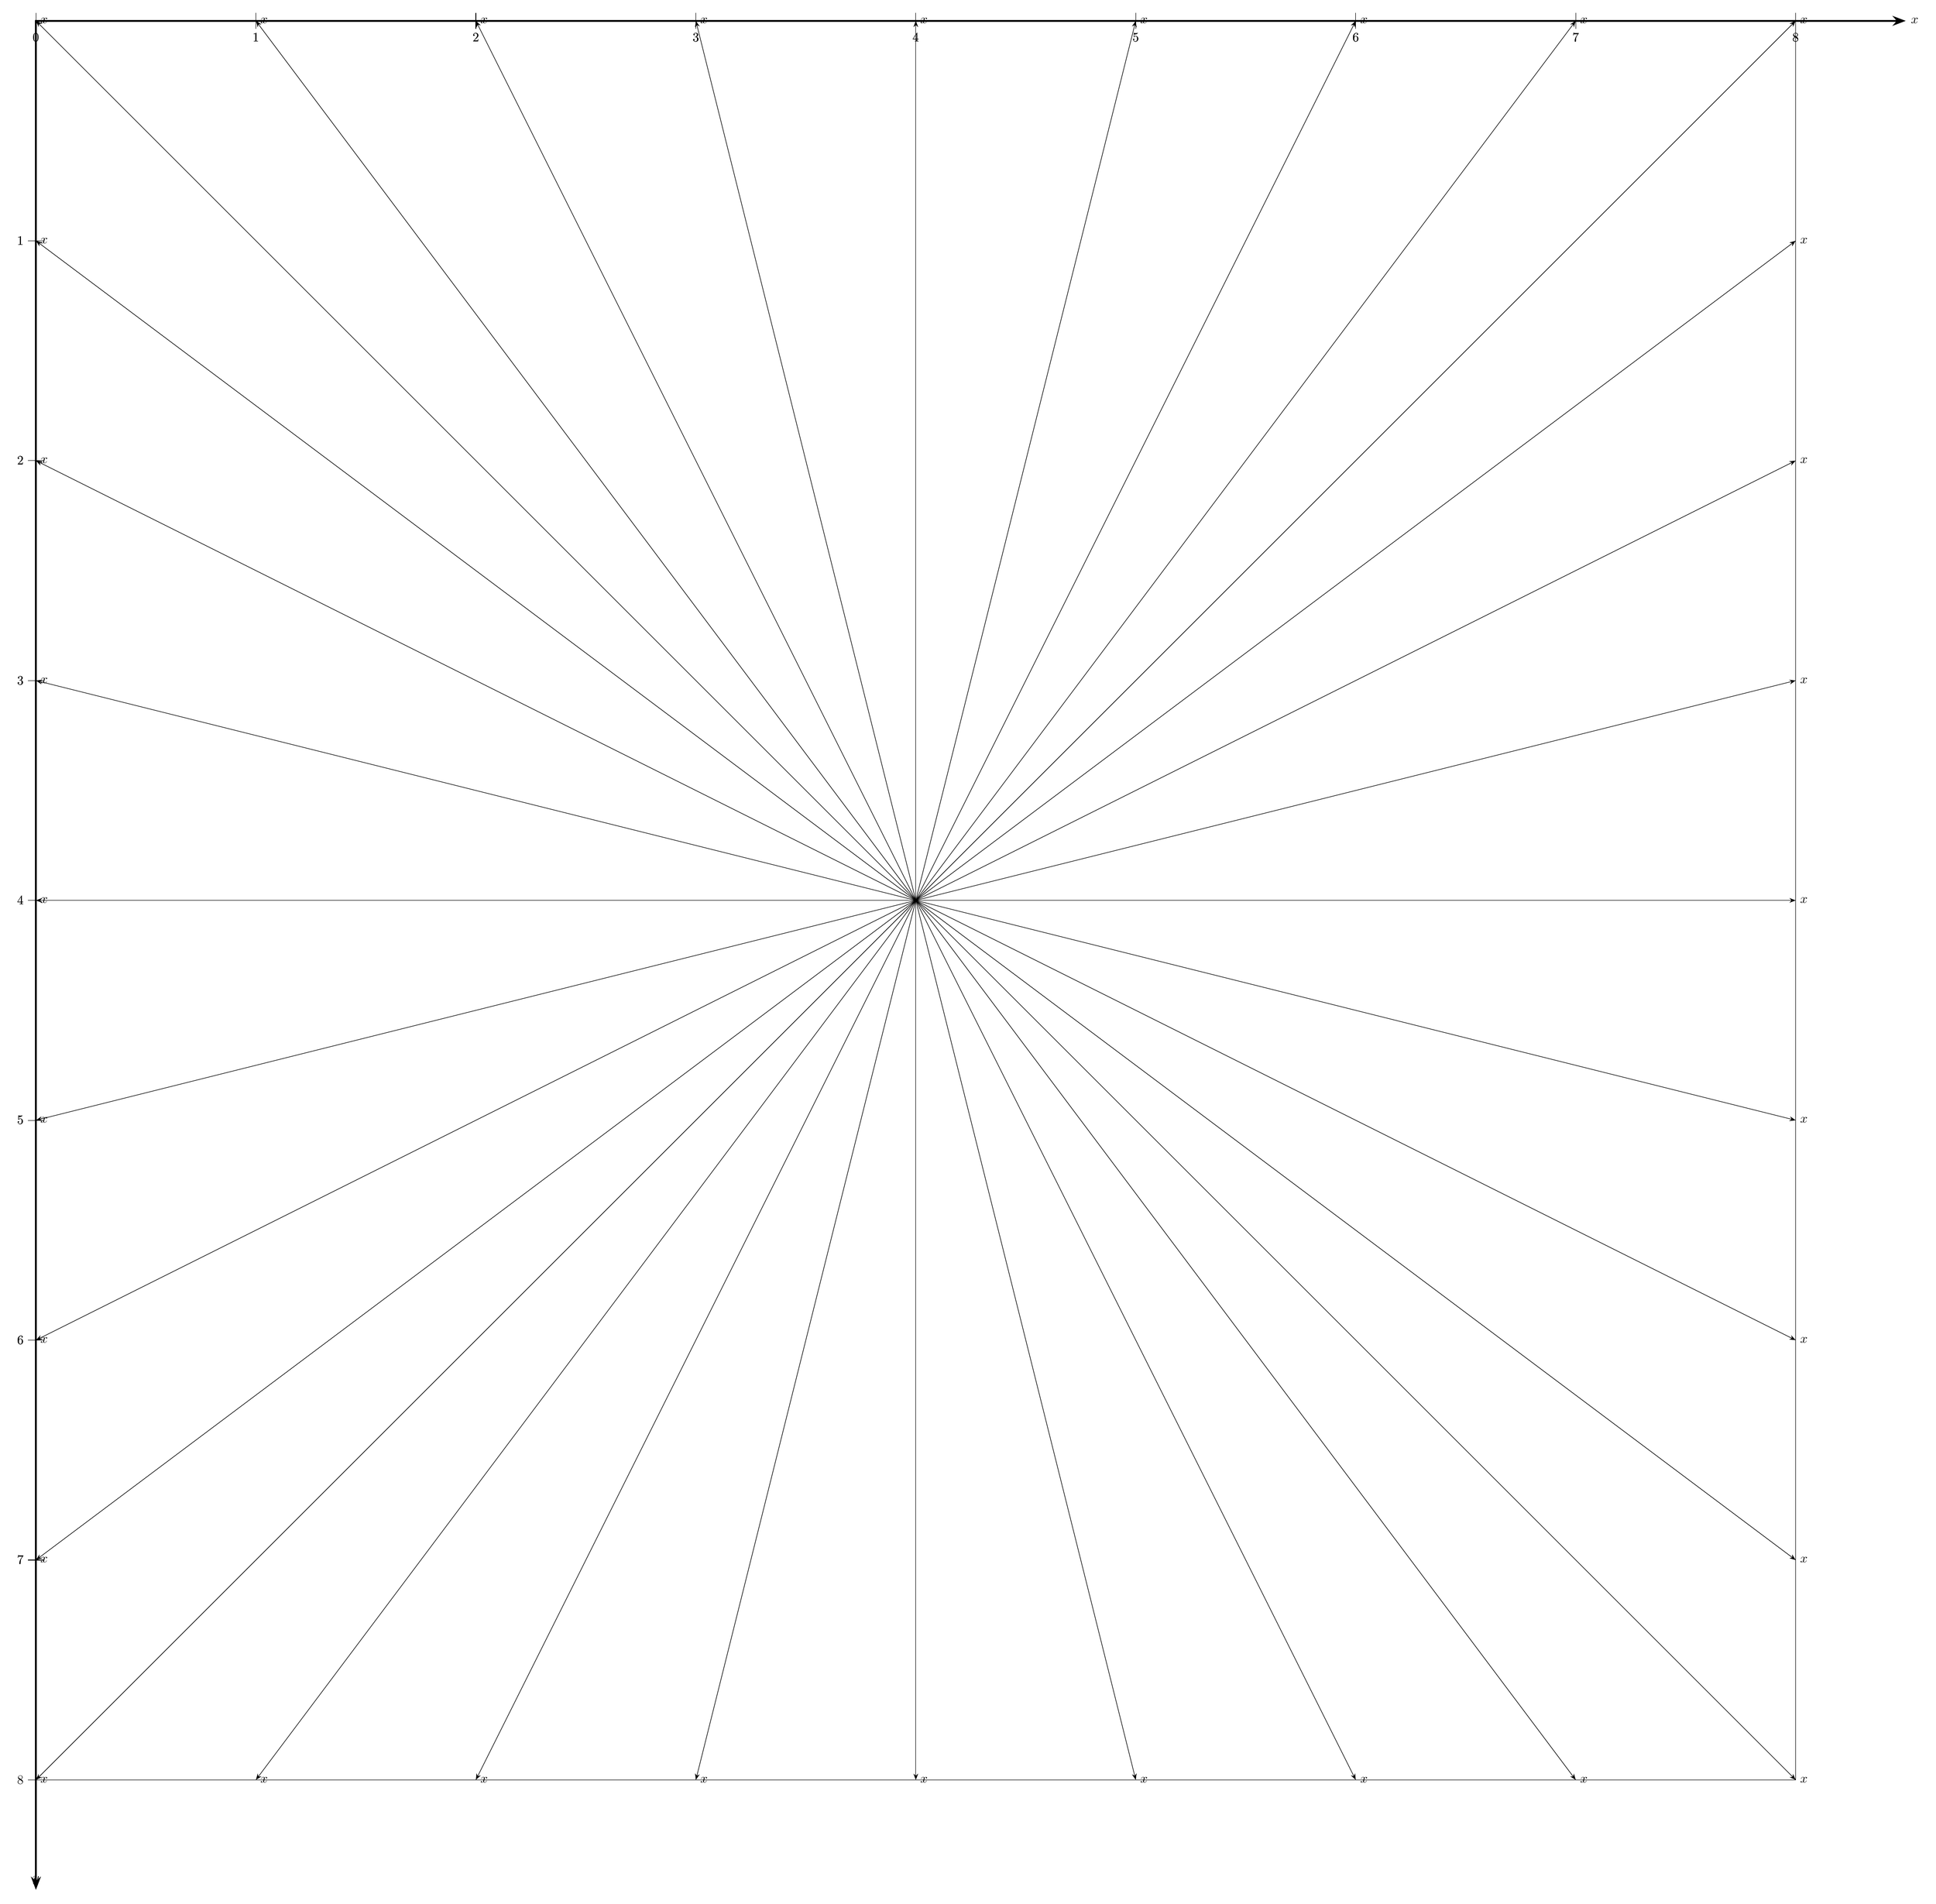
\begin{tikzpicture} 
% Style
[
    scale=6, line cap=round, axes/.style=,
    important line/.style={very thick},
    information text/.style={rounded corners,fill=red!10,inner sep=1ex}
]

%=================================== Start ===================================
{
    % Define: Axis
    %\draw [help lines, step = 1cm] (0, 0) grid (8.0cm, -8.0cm);
    \begin{scope}[axes]
        \draw[->,ultra thick] (0, 0) -- ( 8.5cm, 0) node[right] {$x$} coordinate(x axis);
        \draw[->,ultra thick] (0, 0) -- (0, -8.5cm) node[above] {$y$} coordinate(y axis);
        \foreach \x in {0,...,8} {
            \draw[xshift=\x cm] (0pt, 1pt) -- (0pt, -1pt) node[below] {$\x$};
            \draw[->] (4cm, -4cm)--(\x cm, 0) node[right]{$x$};
        }
        \foreach \y in {1,...,8} {
            \draw[yshift=-\y cm] (1pt, 0pt) -- (-1pt, 0pt) node[left ] {$\y$};
            \draw[->] (4cm, -4cm)--(0,-\y cm) node[right]{$x$};
        }
        \foreach \x in {1,...,8} {
            \draw[xshift=\x cm] (0pt, 1pt) -- (0pt, -1pt) node[below] {$\x$};
            \draw[->] (4cm, -4cm)--(\x cm, -8cm) node[right]{$x$};
        }
        \foreach \y in {1,...,7} {
            \draw[yshift=-\y cm] (1pt, 0pt) -- (-1pt, 0pt) node[left ] {$\y$};
            \draw[->] (4cm, -4cm)--(8cm,-\y cm) node[right]{$x$};
        }
        \draw[-] (0, -8cm) -- (8cm, -8cm);
        \draw[-] (8cm, -8cm) -- (8cm, 0);
    \end{scope}

    % Draw: Circle
    % \draw (0,0) circle [radius = 1cm];
    
    % Draw: Rectangle-90
    % \foo draw_complex_exponential{01} {30} {k}                {1mm}
    % \foo draw_complex_exponential{90} {120}{k+\frac{\pi}{2}}  {2mm}
    % \foo draw_complex_exponential{180}{210}{k+\pi}            {3mm}
    % \foo draw_complex_exponential{270}{300}{k+\frac{3\pi}{2}} {4mm}

    % Draw: Rectangle-180
    % \foo draw_complex_exponential{01} {30} {k}                {1mm}
    % \foo draw_complex_exponential{180}{210}{k+\pi}            {3mm}
}
%==================================== END ====================================

\end{tikzpicture}
\end{document}